\documentclass[11pt]{article}
\usepackage[margin=1in]{geometry}
\usepackage[T1]{fontenc}
\usepackage{lmodern}
\usepackage{amsmath,amssymb,amsthm,bm}
\usepackage{booktabs,multirow,makecell,array}
\usepackage{graphicx}
\usepackage{xcolor}
\usepackage{tikz}
\usetikzlibrary{arrows.meta,positioning,shapes.geometric,fit,calc,decorations.pathreplacing}
\usepackage[numbers,sort&compress]{natbib}
\usepackage[colorlinks=true,linkcolor=blue!50!black,citecolor=blue!50!black,urlcolor=blue!50!black]{hyperref}
\usepackage[capitalise]{cleveref}
\usepackage{caption,subcaption}

\newtheorem{proposition}{Proposition}
\newtheorem{definition}{Definition}
\newcommand{\R}{\mathbb{R}}
\newcommand{\PD}{\mathcal{D}}
\newcommand{\Dist}{\operatorname{Dist}}
\newcommand{\TU}{\operatorname{TU}}
\newcommand{\pTU}{\operatorname{pTU}}
\newcommand{\NP}{\operatorname{NP}}
\newcommand{\SW}{\operatorname{SW}}
\newcommand{\Var}{\operatorname{Var}}
\newcommand{\todo}[1]{\textcolor{red}{[TODO: #1]}}

\tikzset{
  box/.style={draw, rounded corners=2pt, fill=#1!12, minimum height=8mm, align=center, font=\small, inner sep=3pt},
  box/.default=blue,
  arr/.style={-{Latex[length=2mm]}, thick},
  neuron/.style={circle, draw, fill=white, minimum size=3.2mm, inner sep=0pt},
}

\title{Topology of Neural-Network Layers for Out-of-Distribution Detection:\\
A Unified View and Benchmark of Six Topological Approaches}
\author{Dat Bui\\ University of Nebraska--Lincoln \\ \small Draft --- \today}
\date{}

\begin{document}
\maketitle

\begin{abstract}
Deep classifiers are often highly confident on inputs that come from outside their training
distribution. Topological data analysis (TDA) offers an alternative signal: instead of the
network's output confidence, it summarizes the \emph{shape} of the network's internal activity
with persistent homology. Several such approaches have been proposed, but they use different
objects (weight graphs, activation graphs, Bayesian samples, point clouds of activations),
different summaries, and different evaluation protocols. We place six of them in one framework
--- \emph{object $\to$ filtration $\to$ persistence diagram $\to$ score} --- implement all of them
on shared models, and evaluate them as out-of-distribution (OOD) detectors under a common
protocol. Our study has two parts: (i) a controlled study with a Bayesian MLP trained on four
in-distribution datasets (MNIST, Fashion-MNIST, KMNIST, SVHN), each tested against 10--12 OOD
sets grouped into near-OOD, far-OOD and covariate shift; and (ii) the OpenOOD v1.5 CIFAR-10 and
CIFAR-100 benchmarks with the released ResNet-18 checkpoints, where our pipeline reproduces the
published baselines exactly. We find that (1) on the MLPs, topological scores reliably detect the
inputs on which softmax confidence fails, but on the well-trained ResNet-18 no per-image
topological score beats the output-based baselines; (2) no per-image topological score wins on
every dataset, while point-cloud topology on small batches of inputs is strong whenever the
classes are few; (3) simple summaries ($\beta_0$ curves, 0-dimensional features) often beat richer
ones (full persistent-Laplacian spectra, $H_1$ features); and (4) how layers are combined, and
which layers are available, matter as much as the summary itself.
\end{abstract}

\section{Introduction}
\label{sec:intro}
A classifier trained on a fixed set of classes will still produce a prediction for an image
from an unseen class, and often a confident one. Detecting such \emph{out-of-distribution}
(OOD) inputs is a prerequisite for deploying neural networks in safety-critical settings, and
has become a large research area with standardized benchmarks such as OpenOOD
\citep{yang2022openood,zhang2023openood}.

Most post-hoc OOD detectors read a scalar from the network's output or penultimate features:
the maximum softmax probability \citep{hendrycks2017baseline}, an energy \citep{liu2020energy},
a feature-space distance \citep{sun2022knn}. A different line of work asks what the
\emph{topology} of the network's internal activity reveals. Rieck et al.\ \citep{rieck2019neural}
summarize trained weights by the persistent homology of layer graphs; Lacombe et al.\
\citep{lacombe2021topological} build one activation graph per input and layer and compare its
persistence diagram with class-wise references; Yeh and Yang \citep{yeh2025ptu} extend this to
Bayesian networks; persistent Laplacians \citep{wolf2025generalized,jones2025petls,botnan2024nonbranching}
add spectral, geometric information to persistent homology; and Magai and Ayzenberg
\citep{magai2022topology} and Purvine et al.\ \citep{purvine2023cnn} study the topology of point
clouds of hidden activations.

These approaches were proposed with different goals (model selection, uncertainty,
interpretability), objects and evaluation protocols, so it is hard to tell which ideas are useful
for OOD detection. This draft makes three contributions:
\begin{itemize}
  \item \textbf{A unified framework} (\cref{sec:framework}) that writes all six approaches as
  \emph{object $\to$ filtration $\to$ persistence diagram $\to$ score}, with the equations and a
  diagram for each (\cref{sec:methods}).
  \item \textbf{A controlled multi-dataset study} (\cref{sec:phase1}): every approach on the same
  Bayesian MLP trained on four in-distribution (ID) datasets, three seeds each, against near-OOD,
  far-OOD and covariate-shift sets.
  \item \textbf{A benchmark on OpenOOD v1.5} (\cref{sec:phase2}): CIFAR-10 and CIFAR-100 with the
  released ResNet-18 checkpoints, reported next to the published post-hoc methods.
\end{itemize}

\section{Background: persistent homology and persistent Laplacians}
\label{sec:background}

\paragraph{Filtrations and persistence diagrams.}
A \emph{filtration} is a nested family of simplicial complexes $K_{t}\subseteq K_{t'}$ for
$t\le t'$. Persistent homology tracks the $q$-dimensional homology classes ($q=0$: connected
components, $q=1$: loops) through the filtration. A class born at $b$ and dying at $d$ gives a
point $(b,d)$ of the \emph{persistence diagram} $\PD_q$, a multiset in the extended plane; its
\emph{persistence} is $|d-b|$. For a weighted graph $G=(V,E,w)$, the \emph{superlevel
filtration} adds all vertices first and then edges in decreasing order of weight,
\begin{equation}
  G^{(t)} = \bigl(V,\ \{e\in E : w(e)\ge t\}\bigr), \qquad t \text{ decreasing}.
  \label{eq:superlevel}
\end{equation}
Since every vertex exists from the start, only 0-dimensional features change, and each edge that
merges two components contributes one point. These edges are exactly those of a
\emph{maximum spanning tree} (MST) of $G$, so
\begin{equation}
  \PD_0(G) = \bigl\{ w(e) : e \in \mathrm{MST}(G) \bigr\},
  \label{eq:mst}
\end{equation}
a multiset of $|V|-1$ real numbers (the birth of every class is the top of the filtration).
For a point cloud $X=\{x_1,\dots,x_n\}\subset\R^d$, the \emph{Vietoris--Rips} filtration
\begin{equation}
  \mathrm{VR}_\varepsilon(X) = \bigl\{\sigma\subseteq X : \|x_i-x_j\|\le\varepsilon\ \ \forall x_i,x_j\in\sigma\bigr\}
  \label{eq:rips}
\end{equation}
yields diagrams in every dimension; $H_0$ deaths are again MST edge lengths, now of the
Euclidean graph on $X$.

\paragraph{Distances between diagrams.}
The $p$-Wasserstein distance between diagrams matches points optimally, allowing points to be
matched to the diagonal $\Delta$:
\begin{equation}
  W_p(\PD,\PD') = \Bigl(\inf_{\gamma:\PD\cup\Delta\to\PD'\cup\Delta}\ \sum_{u}\|u-\gamma(u)\|_\infty^p\Bigr)^{1/p}.
  \label{eq:wasserstein}
\end{equation}
For the 1-D diagrams of \cref{eq:mst} with a fixed number of points, the optimal matching sorts
both multisets, so $W_2$ is the Euclidean distance between sorted vectors. The \emph{sliced
Wasserstein} distance \citep{carriere2017sliced} averages 1-D Wasserstein distances of projections
onto lines $\ell_\theta$:
\begin{equation}
  \SW(\PD,\PD') = \frac{1}{\pi}\int_{-\pi/2}^{\pi/2} W_1\bigl(\pi_\theta(\PD\cup\pi_\Delta(\PD')),\
  \pi_\theta(\PD'\cup\pi_\Delta(\PD))\bigr)\,d\theta,
  \label{eq:sw}
\end{equation}
where $\pi_\theta$ projects onto $\ell_\theta$ and $\pi_\Delta$ onto the diagonal.
The \emph{Fréchet mean} and \emph{variance} of diagrams $\PD^{(1)},\dots,\PD^{(S)}$ are
\begin{equation}
  \bar\PD=\arg\min_{\PD}\sum_{s}\Dist(\PD^{(s)},\PD)^2,\qquad
  \Var = \frac1S\sum_s \Dist(\PD^{(s)},\bar\PD)^2 .
  \label{eq:frechet}
\end{equation}
For equal-size 1-D diagrams under $W_2$, $\bar\PD$ is the coordinate-wise mean of the sorted vectors.

\paragraph{Persistent Laplacians.}
Let $\partial_q^K$ be the boundary map of a complex $K$ and $\Delta_q^K = \partial_{q+1}^K
\partial_{q+1}^{K\top} + \partial_q^{K\top}\partial_q^K$ its combinatorial Laplacian. For a pair
$K\subseteq L$, let $C_{q+1}^{L,K}=\{c\in C_{q+1}^L : \partial_{q+1}^L c \in C_q^K\}$ and let
$\partial_{q+1}^{L,K}$ be the restriction of $\partial^L_{q+1}$ to it. The \emph{persistent
Laplacian} is \citep{wang2020persistent,memoli2022persistent}
\begin{equation}
  \Delta_q^{K,L} = \underbrace{\partial_{q+1}^{L,K}\bigl(\partial_{q+1}^{L,K}\bigr)^{\!\top}}_{\Delta_{q,\mathrm{up}}^{K,L}}
  + \underbrace{\bigl(\partial_q^{K}\bigr)^{\!\top}\partial_q^{K}}_{\Delta_{q,\mathrm{down}}^{K}} .
  \label{eq:pl}
\end{equation}
Its kernel has dimension equal to the persistent Betti number $\beta_q^{K,L}$, so it contains the
information of persistent homology; its nonzero eigenvalues add geometric information
\citep{memoli2022persistent}. Wolf et al.\ \citep{wolf2025generalized} prove that the up and down
parts are stable while the full operator need not be.

\section{A unified framework}
\label{sec:framework}

\begin{figure}[t]
\centering
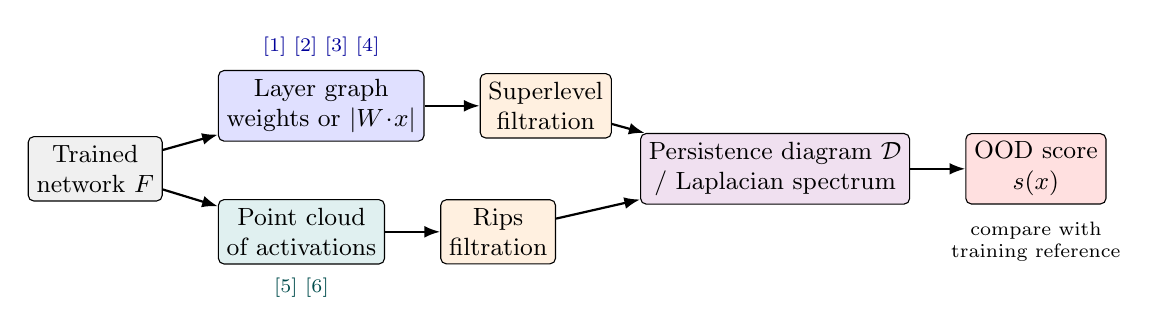
\begin{tikzpicture}[node distance=5mm and 7mm]
  \node[box=gray] (net) {Trained\\network $F$};
  \node[box=blue, right=of net, yshift=8mm] (graph) {Layer graph\\weights or $|W\!\cdot\!x|$};
  \node[box=teal, right=of net, yshift=-8mm] (cloud) {Point cloud\\of activations};
  \node[box=orange, right=of graph] (filtg) {Superlevel\\filtration};
  \node[box=orange, right=of cloud] (filtc) {Rips\\filtration};
  \node[box=violet, right=15mm of $(filtg)!0.5!(filtc)$] (pd) {Persistence diagram $\PD$\\ / Laplacian spectrum};
  \node[box=red, right=of pd] (score) {OOD score\\$s(x)$};
  \draw[arr] (net) -- (graph); \draw[arr] (net) -- (cloud);
  \draw[arr] (graph) -- (filtg); \draw[arr] (cloud) -- (filtc);
  \draw[arr] (filtg) -- (pd); \draw[arr] (filtc) -- (pd); \draw[arr] (pd) -- (score);
  \node[font=\scriptsize, align=center, below=1mm of score] {compare with\\training reference};
  \node[font=\scriptsize, text=blue!60!black, above=0.5mm of graph] {[1] [2] [3] [4]};
  \node[font=\scriptsize, text=teal!60!black, below=0.5mm of cloud] {[5] [6]};
\end{tikzpicture}
\caption{All six approaches follow one pipeline: build an object from the network, filter it,
summarize it with a persistence diagram (or a persistent-Laplacian spectrum), and turn the
summary into an OOD score by comparing it with what training data produce.}
\label{fig:framework}
\end{figure}

\Cref{fig:framework} shows the common structure. Let $F:\R^{h_0}\to\R^{K}$ be an $L$-layer
network, $x_\ell$ the input of layer $\ell$ (so $x_0=x$), and $W_\ell\in\R^{h_\ell\times
h_{\ell-1}}$ its weights. The approaches differ in (a) the object: a bipartite layer graph or a
point cloud; (b) whether the object depends on the input $x$; and (c) how the diagram becomes a
score. \Cref{tab:taxonomy} summarizes them; \cref{sec:methods} gives the details.

\begin{table}[t]
\centering
\resizebox{\linewidth}{!}{%
\begin{tabular}{@{}lllll@{}}
\toprule
& Object & Depends on $x$? & Summary & OOD score \\
\midrule
{[1]} NP \citep{rieck2019neural} & graph of $|W_\ell|$ & no & $\|\PD_0\|_p$ & (input-dependent variant, \S\ref{sec:np}) \\
{[2]} TU \citep{lacombe2021topological} & graph of $|W_\ell\,x_{\ell-1}|$ & yes & $\PD_0$ (MST) & $W_2$ to class-mean $\PD_0$ \\
{[3]} pTU \citep{yeh2025ptu} & same, $S$ posterior samples & yes & $\PD_0$ & Fréchet variance; permutation test \\
{[4]} PL \citep{wolf2025generalized} & thresholded activation graph & yes & spectrum of $\Delta_0^{K,L}$ & distance to class-mean spectrum \\
{[5]} Manifold \citep{magai2022topology} & point cloud per layer & set of inputs & $H_0,H_1$, intrinsic dim. & batch descriptors; local $\Delta H_0$ \\
{[6]} CNN act.\ \citep{purvine2023cnn} & point cloud per layer & set of inputs & $\PD_0,\PD_1$ & SW to reference; layer profile \\
\bottomrule
\end{tabular}}
\caption{The six approaches in the framework of \cref{fig:framework}.}
\label{tab:taxonomy}
\end{table}

\section{The six approaches}
\label{sec:methods}

\subsection{[1] Neural persistence}
\label{sec:np}
\begin{figure}[h]
\centering
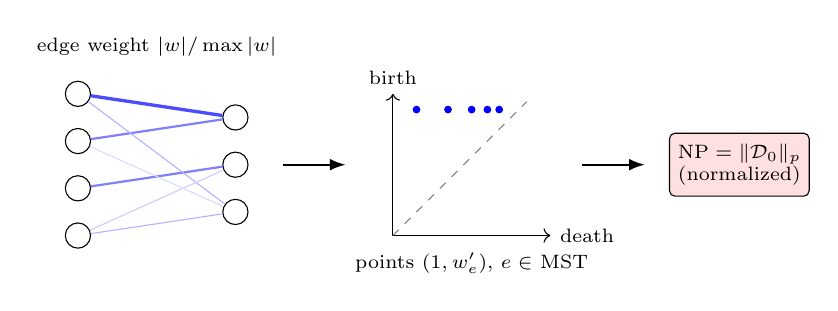
\begin{tikzpicture}[x=1cm,y=1cm]
  \foreach \i in {0,...,3} \node[neuron] (a\i) at (0,-\i*0.6) {};
  \foreach \j in {0,...,2} \node[neuron] (b\j) at (2,-0.3-\j*0.6) {};
  \draw[very thick, blue!70] (a0)--(b0); \draw[thick, blue!50] (a2)--(b1); \draw[thick, blue!50] (a1)--(b0);
  \draw[blue!30] (a3)--(b2); \draw[blue!30] (a0)--(b2); \draw[blue!20] (a3)--(b1); \draw[blue!15] (a1)--(b2);
  \node[font=\scriptsize, align=center] at (1,0.6) {edge weight $|w|/\max|w|$};
  \draw[arr] (2.6,-0.9) -- (3.4,-0.9);
  \begin{scope}[shift={(4,-1.8)}]
    \draw[->] (0,0) -- (2,0) node[right,font=\scriptsize] {death};
    \draw[->] (0,0) -- (0,1.8) node[above,font=\scriptsize] {birth};
    \draw[dashed,gray] (0,0) -- (1.7,1.7);
    \foreach \d in {0.3,0.7,1.0,1.2,1.35} \fill[blue] (\d,1.6) circle (1.4pt);
    \node[font=\scriptsize] at (1,-0.35) {points $(1,w'_e)$, $e\in$ MST};
  \end{scope}
  \draw[arr] (6.4,-0.9) -- (7.2,-0.9);
  \node[box=red, font=\scriptsize] at (8.4,-0.9) {$\NP=\|\PD_0\|_p$\\(normalized)};
\end{tikzpicture}
\caption{[1] Neural persistence: a layer of trained weights as a bipartite graph, its 0-dimensional
diagram (the MST weights), and the $p$-norm of the diagram.}
\label{fig:np}
\end{figure}
Rieck et al.\ \citep{rieck2019neural} view layer $\ell$ as the complete bipartite graph
$G_\ell=(V_{\ell-1}\sqcup V_\ell,E_\ell)$ with weights normalized over the whole network,
\begin{equation}
  w'(i,j) = \frac{|W_\ell(j,i)|}{\max_{\ell',i',j'}|W_{\ell'}(j',i')|}\in[0,1].
\end{equation}
Under the superlevel filtration (\cref{eq:superlevel}) every vertex is born at $1$ and every MST
edge $e$ kills a component at $w'_e$, giving $\PD_0(G_\ell)=\{(1,w'_e)\}$. Neural persistence is
\begin{equation}
  \NP(G_\ell) = \|\PD_0(G_\ell)\|_p = \Bigl(\sum_{e\in\mathrm{MST}(G_\ell)} (1-w'_e)^p\Bigr)^{1/p},
  \qquad 0\le \NP(G_\ell)\le (1-\min_e w'_e)\,(|V_\ell|-1)^{1/p},
  \label{eq:np}
\end{equation}
normalized by the upper bound and averaged over layers. $\NP$ depends only on the weights, so it
assigns the same value to every input and cannot rank inputs (AUROC $=50$ by construction).
\emph{Adaptation.} We apply \cref{eq:np} to the input-dependent activation graph of [2]
(\cref{eq:actgraph}) and score $s(x)=|\NP(x)-\mu_{k}|/\sigma_{k}$, where $(\mu_k,\sigma_k)$ are the
training statistics of the predicted class $k=\arg\max F(x)$.

\subsection{[2] Topological uncertainty}
\begin{figure}[h]
\centering
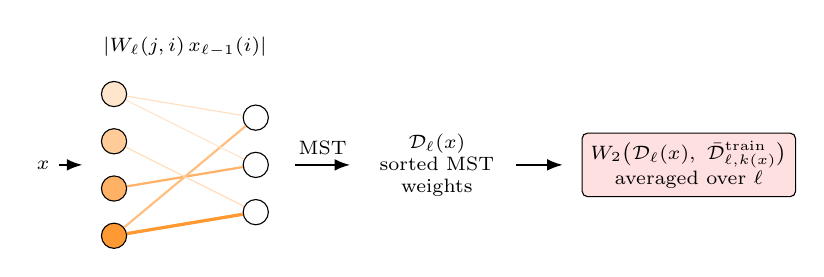
\begin{tikzpicture}[x=1cm,y=1cm]
  \node[font=\scriptsize] at (-0.6,-0.9) {$x$};
  \draw[arr] (-0.4,-0.9) -- (-0.1,-0.9);
  \foreach \i in {0,...,3} \node[neuron, fill=orange!\the\numexpr 20+20*\i\relax] (a\i) at (0.3,-\i*0.6) {};
  \foreach \j in {0,...,2} \node[neuron] (b\j) at (2.1,-0.3-\j*0.6) {};
  \draw[very thick, orange!80] (a3)--(b2); \draw[thick, orange!60] (a2)--(b1); \draw[thick, orange!50] (a3)--(b0);
  \draw[orange!25] (a0)--(b0); \draw[orange!30] (a1)--(b2); \draw[orange!20] (a0)--(b1);
  \node[font=\scriptsize] at (1.2,0.6) {$|W_\ell(j,i)\,x_{\ell-1}(i)|$};
  \draw[arr] (2.6,-0.9) -- (3.3,-0.9) node[midway,above,font=\scriptsize] {MST};
  \node[font=\scriptsize, align=center] at (4.4,-0.9) {$\PD_\ell(x)$\\sorted MST\\weights};
  \draw[arr] (5.4,-0.9) -- (6.0,-0.9);
  \node[box=red, font=\scriptsize] at (7.6,-0.9) {$W_2\bigl(\PD_\ell(x),\ \bar\PD_{\ell,k(x)}^{\mathrm{train}}\bigr)$\\averaged over $\ell$};
\end{tikzpicture}
\caption{[2] Topological uncertainty: one activation graph per input and layer; its diagram is
compared with the Fréchet mean of training diagrams of the predicted class.}
\label{fig:tu}
\end{figure}
Lacombe et al.\ \citep{lacombe2021topological} weight the edges of layer $\ell$ by how much input
$x$ uses them,
\begin{equation}
  w_x(i,j) = |W_\ell(j,i)\,x_{\ell-1}(i)| ,
  \label{eq:actgraph}
\end{equation}
which gives one \emph{activation graph} $G_\ell(x)$ per input and layer. Its diagram
$\PD_\ell(x)$ is the multiset of its $N_\ell=h_{\ell-1}+h_\ell-1$ MST weights (\cref{eq:mst}). For
each class $k$, the reference $\bar\PD^{\mathrm{train}}_{\ell,k}$ is the Fréchet mean
(\cref{eq:frechet}) of the training diagrams predicted as $k$, and
\begin{equation}
  \TU(x) = \frac{1}{L}\sum_{\ell=1}^{L} W_2\bigl(\PD_\ell(x),\ \bar\PD^{\mathrm{train}}_{\ell,k(x)}\bigr),
  \qquad k(x)=\arg\max_k F(x)_k .
  \label{eq:tu}
\end{equation}
\emph{Variant (ours).} The layer distances live on different scales, so the plain average is
dominated by the largest. \emph{TU-rescaled} divides each layer's distance by its mean over
training inputs before averaging.

\subsection{[3] Predictive topological uncertainty}
\begin{figure}[h]
\centering
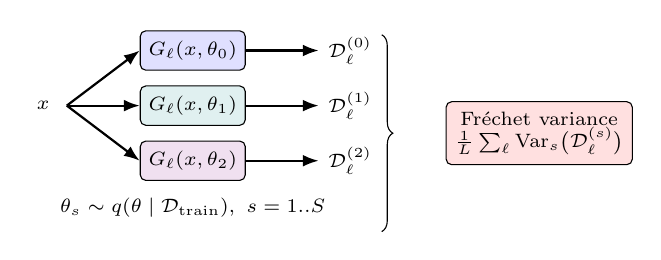
\begin{tikzpicture}[x=1cm,y=1cm]
  \node[font=\scriptsize] at (-0.3,0) {$x$};
  \foreach \s/\c in {0/blue,1/teal,2/violet} {
    \node[box=\c, font=\scriptsize, minimum height=5mm] (g\s) at (1.6,0.7-\s*0.7) {$G_\ell(x,\theta_{\s})$};
    \draw[arr] (0,0) -- (g\s.west);
    \node[font=\scriptsize] (d\s) at (3.6,0.7-\s*0.7) {$\PD_\ell^{(\s)}$};
    \draw[arr] (g\s.east) -- (d\s.west);
  }
  \node[font=\scriptsize] at (1.6,-1.3) {$\theta_s\sim q(\theta\mid\mathcal{D}_{\mathrm{train}}),\ s=1..S$};
  \draw[decorate,decoration={brace,amplitude=4pt}] (4.0,0.9) -- (4.0,-1.6);
  \node[box=red, font=\scriptsize] at (6.0,-0.35) {Fréchet variance\\$\frac1L\sum_\ell\Var_s\bigl(\PD_\ell^{(s)}\bigr)$};
\end{tikzpicture}
\caption{[3] pTU: the activation-graph diagrams of $S$ posterior samples of a Bayesian network;
their spread is the uncertainty.}
\label{fig:ptu}
\end{figure}
For a Bayesian network with (approximate) posterior $q(\theta\mid\mathcal{D}_{\mathrm{train}})$,
Yeh and Yang \citep{yeh2025ptu} draw $\theta_1,\dots,\theta_S$ and build $G_\ell(x,\theta_s)$ as in
\cref{eq:actgraph}, each with diagram $\PD^{(s)}_\ell(x)$. The predictive topological uncertainty is
the posterior Fréchet variance averaged over layers,
\begin{equation}
  \pTU(x) = \frac1L\sum_{\ell=1}^{L} \frac1S\sum_{s=1}^{S} W_2\bigl(\PD_\ell^{(s)}(x),\ \bar\PD_\ell(x)\bigr)^2 .
  \label{eq:ptu}
\end{equation}
At the dataset level, the paper tests $H_0: P_{\mathrm{test}}=P_{\mathrm{train}}$ with a
permutation test whose statistic is the empirical Wasserstein distance between the pTU values of
$m$ training and $m$ test inputs,
$T = \bigl(\sum_{i=1}^{m}|Y_{(i)}-Z_{(i)}|^p\bigr)^{1/p}$, with order statistics $Y_{(i)},Z_{(i)}$.
\emph{Posterior.} For the MLP we train with Bayes-by-Backprop \citep{blundell2015weight}; for the
ResNet-18 checkpoints we use a diagonal last-layer Laplace approximation
\citep{daxberger2021laplace}, $q(W)=\mathcal{N}\bigl(W^\star,\,(\tau I+\mathrm{diag}\,\mathrm{GGN})^{-1}\bigr)$,
with the prior precision $\tau$ chosen on the validation set. \emph{Variant (ours).}
\emph{pTU two-sided} scores $|\log\pTU(x)-\mathrm{median}_{\mathrm{train}}\log\pTU|$, because we
find that OOD inputs can have \emph{lower} pTU than training data.

\subsection{[4] Persistent Laplacian}
\begin{figure}[h]
\centering
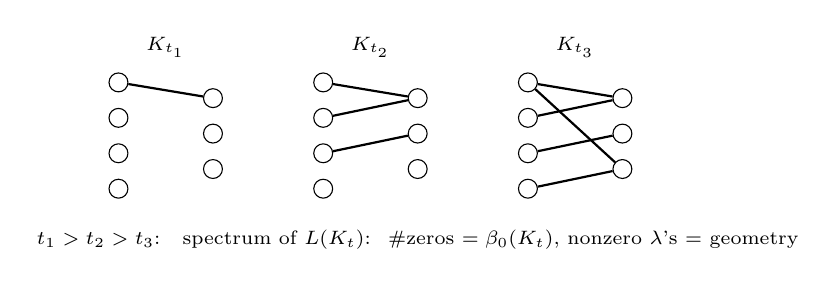
\begin{tikzpicture}[x=1cm,y=1cm]
  \foreach \t/\xo/\lab in {0/0/{t_1},1/2.6/{t_2},2/5.2/{t_3}} {
    \begin{scope}[shift={(\xo,0)}]
      \foreach \i in {0,...,3} \node[neuron, minimum size=2.4mm] (a\t\i) at (0,-\i*0.45) {};
      \foreach \j in {0,...,2} \node[neuron, minimum size=2.4mm] (b\t\j) at (1.2,-0.2-\j*0.45) {};
      \node[font=\scriptsize] at (0.6,0.45) {$K_{\lab}$};
    \end{scope}
  }
  \draw[thick] (a00)--(b00);
  \draw[thick] (a10)--(b10); \draw[thick] (a12)--(b11); \draw[thick] (a11)--(b10);
  \draw[thick] (a20)--(b20); \draw[thick] (a22)--(b21); \draw[thick] (a21)--(b20); \draw[thick] (a23)--(b22); \draw[thick] (a20)--(b22);
  \node[font=\scriptsize, align=center] at (3.8,-2.0) {$t_1>t_2>t_3$:\quad spectrum of $L(K_t)$: \ \#zeros $=\beta_0(K_t)$, nonzero $\lambda$'s = geometry};
\end{tikzpicture}
\caption{[4] Persistent Laplacian on the activation graph: in dimension 0 with all vertices born
first, $\Delta_0^{K_s,K_t}$ is the graph Laplacian of $K_t$.}
\label{fig:pl}
\end{figure}
\begin{proposition}
\label{prop:pl}
Let $K_t$ be the superlevel filtration (\cref{eq:superlevel}) of a graph whose vertices are all
present at the start. For $K_s\subseteq K_t$, $\Delta_0^{K_s,K_t} = L(K_t) = D_t - A_t$, the
combinatorial graph Laplacian of $K_t$. For a bipartite graph, $\Delta_q^{K_s,K_t}=0$ for $q\ge1$.
\end{proposition}
\begin{proof}[Sketch]
$\Delta_{0,\mathrm{down}}=0$ since $\partial_0=0$. Every edge of $K_t$ has both endpoints in
$V=V(K_s)$, so $C_1^{K_t,K_s}=C_1^{K_t}$ and $\Delta_{0,\mathrm{up}}^{K_s,K_t}=\partial_1^{K_t}\partial_1^{K_t\top}=L(K_t)$.
A bipartite graph has no triangles, so there are no 2-simplices and no 1-cycles bound by them.
\end{proof}
Hence the zero eigenvalues of $L(K_t)$ count $\beta_0(K_t)$, which is the information of the
diagram of [2], while the nonzero eigenvalues are what the persistent Laplacian adds. For three
thresholds $t$ (quantiles of training MST weights) we use
$\phi_t(x)=\bigl(\beta_0,\ |E(K_t)|,\ \lambda_{\min}^{+},\ \lambda_{\max},\ \mathrm{std}(\lambda^{+})\bigr)$
and score
\begin{equation}
  s_{\mathrm{PL}}(x) = \frac{1}{|\mathcal{T}|\,|\phi|}\sum_{\ell,t}\Bigl\|\frac{\phi_{\ell,t}(x)-\mu_{\ell,t,k(x)}}{\sigma_{\ell,t}}\Bigr\|_2^2 ,
  \label{eq:pl-score}
\end{equation}
with class-wise means $\mu$ and standard deviations $\sigma$ from training data. Using only the
$\beta_0$ coordinate isolates the persistent-homology part.

\subsection{[5] Topology and geometry of the data manifold}
\begin{figure}[h]
\centering
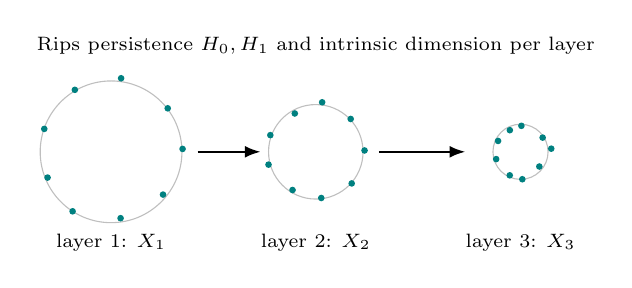
\begin{tikzpicture}[x=1cm,y=1cm]
  \foreach \l/\xo/\r in {1/0/0.9,2/2.6/0.6,3/5.2/0.35} {
    \begin{scope}[shift={(\xo,0)}]
      \draw[gray!50] (0,0) circle (\r);
      \foreach \a in {0,40,...,320} \fill[teal] ({\r*cos(\a)+0.05*rand},{\r*sin(\a)+0.05*rand}) circle (1.2pt);
      \node[font=\scriptsize] at (0,-1.15) {layer \l: $X_\l$};
    \end{scope}
  }
  \draw[arr] (1.1,0) -- (1.9,0); \draw[arr] (3.4,0) -- (4.5,0);
  \node[font=\scriptsize, align=center] at (2.6,1.35) {Rips persistence $H_0,H_1$ and intrinsic dimension per layer};
\end{tikzpicture}
\caption{[5] Each layer maps a set of inputs to a point cloud; its topology and dimension are
tracked across layers.}
\label{fig:manifold}
\end{figure}
For inputs $x_1,\dots,x_n$ and layer $\ell$, Magai and Ayzenberg \citep{magai2022topology} study
$X_\ell=\{h_\ell(x_1),\dots,h_\ell(x_n)\}\subset\R^{h_\ell}$ (for convolutional layers, spatially
averaged), its Rips diagrams $\PD_0,\PD_1$ (\cref{eq:rips}), the \emph{total persistence}
$P_q(X_\ell)=\sum_{(b,d)\in\PD_q}(d-b)$ and an intrinsic-dimension estimate; we use TwoNN
\citep{facco2017twonn},
\begin{equation}
  \hat m(X) = \frac{n}{\sum_{i=1}^{n}\log\bigl(r_2(x_i)/r_1(x_i)\bigr)},
  \label{eq:twonn}
\end{equation}
with $r_1,r_2$ the distances to the two nearest neighbours. \emph{Batch score.} A batch of $m$
inputs gives $\psi=\bigl(P_0,P_1,\hat m\bigr)_{\ell=1..L}$, scored by its mean squared $z$-score
against training batches of the same size. \emph{Per-image adaptation (ours).} For an input $x$
let $N_k(x)$ be its $k$ nearest training points in layer $\ell$; the local change
\begin{equation}
  \Delta P_0^{\ell}(x) = P_0\bigl(N_k(x)\cup\{h_\ell(x)\}\bigr) - P_0\bigl(N_k(x)\bigr)
  \label{eq:local}
\end{equation}
is the increase of the minimum-spanning-tree length when $x$ joins its neighbourhood; the score
is the mean squared $z$-score of $(\Delta P_0^{\ell})_\ell$.

\subsection{[6] Topology of CNN activations}
\begin{figure}[h]
\centering
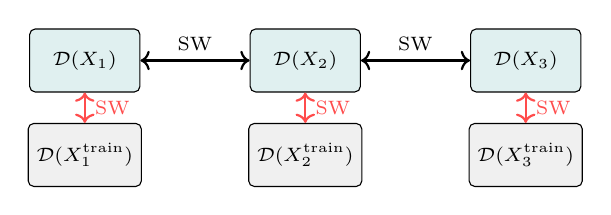
\begin{tikzpicture}[x=1cm,y=1cm]
  \foreach \l/\xo in {1/0,2/2.8,3/5.6} {
    \node[box=teal, font=\scriptsize, minimum width=1.4cm] (p\l) at (\xo,0) {$\PD(X_\l)$};
  }
  \draw[<->, thick] (p1) -- (p2) node[midway,above,font=\scriptsize] {$\SW$};
  \draw[<->, thick] (p2) -- (p3) node[midway,above,font=\scriptsize] {$\SW$};
  \foreach \l/\xo in {1/0,2/2.8,3/5.6} {
    \node[box=gray, font=\scriptsize, minimum width=1.4cm] (r\l) at (\xo,-1.2) {$\PD(X^{\mathrm{train}}_\l)$};
    \draw[<->, thick, red!70] (p\l) -- (r\l) node[midway,right,font=\scriptsize] {$\SW$};
  }
\end{tikzpicture}
\caption{[6] Diagrams of every layer, compared across layers (Purvine et al.'s layer profile) and
with reference diagrams of training batches (our OOD score).}
\label{fig:sw}
\end{figure}
Purvine et al.\ \citep{purvine2023cnn} represent each image at a convolutional layer by the channel
vector at the spatial position of largest activation norm, compute the Rips diagrams of the
resulting point cloud, and compare layers with the sliced Wasserstein distance (\cref{eq:sw}).
We use two batch scores: the distance to reference diagrams,
$s_{\SW}(B)=\frac{1}{2L}\sum_{\ell,q}z\bigl(\frac1R\sum_{r}\SW(\PD_q(X_\ell^{B}),\PD_q(X_\ell^{r}))\bigr)$
over $R$ training batches, and the \emph{layer profile}
$\bigl(\SW(\PD_q(X_\ell^B),\PD_q(X_{\ell+1}^B))\bigr)_{\ell,q}$ scored by its squared $z$-score.

\section{Experimental protocol}
\label{sec:protocol}
\paragraph{Metrics.} Following OpenOOD \citep{zhang2023openood}, OOD is the positive class. We report
AUROC and FPR@95 (the fraction of ID inputs flagged at the threshold that detects 95\% of OOD
inputs); each is computed per OOD set and averaged within the near-OOD and far-OOD groups. All
numbers are means (± std) over three training seeds or checkpoints.
\paragraph{Per-image and batch settings.} The standard setting scores one input at a time. Since
[3], [5] and [6] are defined on sets of inputs, we also score batches of $m\in\{10,20\}$ inputs
drawn from a single source and report AUROC over batches.
\paragraph{Baselines.} MSP \citep{hendrycks2017baseline}, energy (EBO) \citep{liu2020energy}, max
logit (MLS) \citep{hendrycks2022scaling}, KNN \citep{sun2022knn}, ViM \citep{wang2022vim}, and the
Bayesian mutual information of the predictive distribution.

\section{Part I: a controlled study across in-distribution datasets}
\label{sec:phase1}
\paragraph{Setup.} We use the Bayesian MLP 784--64--16--10 of \citep{yeh2025ptu}, trained with
Bayes-by-Backprop (scale-mixture prior $\sigma_1=1,\sigma_2=0.007$, KL term scaled by $0.1$, early
stopping with patience 25), on four ID datasets, all grayscale $28\times28$ in $[0,1]$. OOD sets
come from OpenOOD's MNIST benchmark (NotMNIST, Fashion-MNIST, Textures, CIFAR-10, TinyImageNet,
Places365) plus SVHN, KMNIST, Gaussian and uniform noise; covariate-shift sets are MNIST-C
\citep{mu2019mnistc} and pixel-flip corruptions \citep{lacombe2021topological}. \Cref{tab:p1-sets}
lists the groups.

\begin{table}[t]
\centering\small
\begin{tabular}{@{}l>{\raggedright}p{3.4cm}>{\raggedright}p{6.2cm}p{3.2cm}@{}}
\toprule
ID set & near-OOD & far-OOD & covariate shift \\
\midrule
MNIST & NotMNIST, F-MNIST, KMNIST & CIFAR10, SVHN, Textures, TIN, Places365, Gaussian, Uniform & MNIST-flip, MNIST-C \tabularnewline
F-MNIST & MNIST, KMNIST, NotMNIST & CIFAR10, SVHN, Textures, TIN, Places365, Gaussian, Uniform & F-MNIST-flip \tabularnewline
KMNIST & MNIST, F-MNIST, NotMNIST & CIFAR10, SVHN, Textures, TIN, Places365, Gaussian, Uniform & KMNIST-flip \tabularnewline
SVHN & CIFAR10, TIN & Places365, Textures, F-MNIST, KMNIST, NotMNIST, Gaussian, Uniform & MNIST, SVHN-flip \tabularnewline
\bottomrule
\end{tabular}
\caption{Part I: OOD sets for each in-distribution set (2000 test images each).}
\label{tab:p1-sets}
\end{table}

\begin{table*}[t]
\centering
\setlength{\tabcolsep}{3pt}\scriptsize
\begin{tabular}{@{}lccccccccccccccc@{}}
\toprule
 & \multicolumn{3}{c}{MNIST (97.2\%)} & \multicolumn{3}{c}{F-MNIST (87.2\%)} & \multicolumn{3}{c}{KMNIST (85.3\%)} & \multicolumn{3}{c}{SVHN (66.8\%)} & \multicolumn{3}{c}{Mean over ID sets} \\
\cmidrule(lr){2-4}\cmidrule(lr){5-7}\cmidrule(lr){8-10}\cmidrule(lr){11-13}\cmidrule(lr){14-16}
Method & Near & Far & Shift & Near & Far & Shift & Near & Far & Shift & Near & Far & Shift & Near & Far & Shift \\
\midrule
{MSP} & 74.1 & 69.2 & 75.3 & 72.2 & 48.3 & 66.3 & 73.4 & 72.6 & 71.9 & 60.2 & 61.4 & 46.4 & 70.0 & 62.9 & 65.0 \\
{Mutual information} & 80.9 & 78.6 & 79.3 & 80.9 & 57.7 & 81.0 & \textbf{76.0} & 77.3 & 77.5 & 66.7 & 61.1 & 50.8 & 76.1 & 68.7 & 72.2 \\
{$k$-NN distance$^\dagger$} & 89.6 & 90.6 & 78.1 & 91.5 & 87.7 & 95.8 & 65.2 & 73.6 & 75.6 & 75.4 & \textbf{89.3} & 83.6 & 80.4 & 85.3 & 83.3 \\
\midrule
{[1] NP (per input)} & 59.2 & 53.5 & 57.0 & 72.4 & 63.8 & 68.7 & 55.8 & 51.8 & 56.4 & 51.0 & 53.8 & 51.4 & 59.6 & 55.7 & 58.4 \\
{[2] TU} & 80.7 & 82.6 & 65.3 & 81.6 & 72.9 & 66.9 & 71.2 & 80.4 & 61.4 & 50.9 & 67.1 & 67.6 & 71.1 & 75.8 & 65.3 \\
{[2] TU-rescaled} & 85.5 & 93.5 & 71.6 & 83.5 & 77.8 & 71.1 & 75.8 & \textbf{90.5} & 67.8 & 49.4 & 69.3 & 67.9 & 73.5 & 82.8 & 69.6 \\
{[3] pTU} & 87.0 & 84.3 & 75.0 & 47.2 & 63.6 & 75.0 & 55.9 & 68.6 & 75.0 & 63.9 & 59.4 & 59.2 & 63.5 & 69.0 & 71.0 \\
{[4] PL, full spectrum$^\dagger$} & 84.1 & 83.1 & 70.8 & 83.5 & 77.0 & 65.7 & 74.5 & 79.2 & 67.9 & 44.9 & 64.8 & 67.4 & 71.7 & 76.0 & 67.9 \\
{[4] PL, $\beta_0$ only$^\dagger$} & 86.1 & 84.6 & 75.5 & 77.7 & 77.1 & 64.5 & 73.5 & 79.7 & 74.3 & 44.4 & 62.4 & 65.6 & 70.4 & 75.9 & 70.0 \\
{[5] local $\Delta H_0$$^\dagger$} & \textbf{96.1} & \textbf{97.0} & \textbf{84.3} & \textbf{96.2} & \textbf{92.4} & \textbf{98.7} & 67.7 & 78.0 & \textbf{89.3} & \textbf{78.2} & 89.2 & \textbf{84.1} & \textbf{84.6} & \textbf{89.2} & \textbf{89.1} \\
\bottomrule
\end{tabular}
\caption{Part I, per-image OOD detection: AUROC (\%, mean over 3 seeds), averaged within each OOD group. ID test accuracy in parentheses. The first three rows are baselines; bold = best in the column. $^\dagger$ = first 1000 images per set. Standard deviations and FPR@95 are in the repository.}
\label{tab:p1-main}
\end{table*}


\begin{figure}[t]
\centering
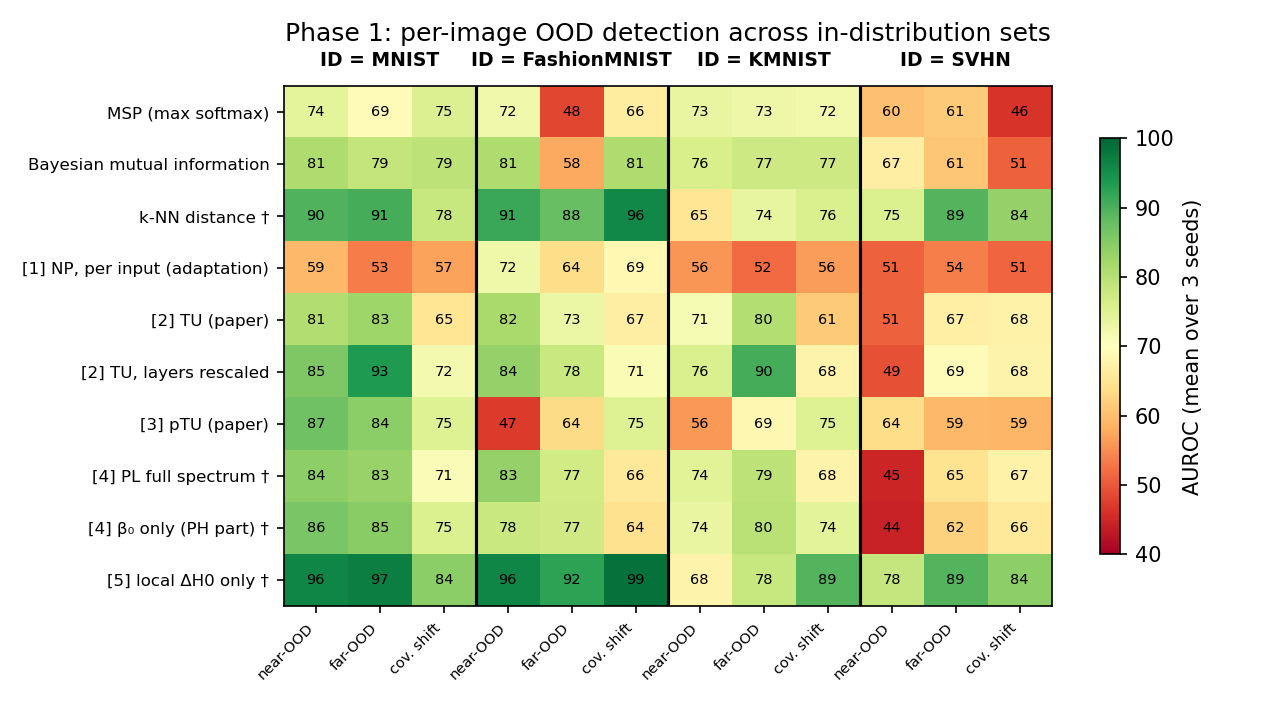
\includegraphics[width=\linewidth]{figures/summary_phase1.png}
\caption{Per-image AUROC of every approach for each ID dataset and OOD group (mean over 3 seeds).}
\label{fig:p1-heat}
\end{figure}

\begin{table}[t]
\centering
\setlength{\tabcolsep}{2.5pt}\scriptsize
\begin{tabular}{@{}clcccccccccccc@{}}
\toprule
 & & \multicolumn{3}{c}{MNIST} & \multicolumn{3}{c}{F-MNIST} & \multicolumn{3}{c}{KMNIST} & \multicolumn{3}{c}{SVHN} \\
\cmidrule(lr){3-5}\cmidrule(lr){6-8}\cmidrule(lr){9-11}\cmidrule(lr){12-14}
$m$ & Method & N & F & S & N & F & S & N & F & S & N & F & S \\
\midrule
\multirow{5}{*}{10} & {MSP (batch mean)} & 93 & 79 & \textbf{93} & 91 & 33 & 89 & 90 & 86 & 91 & 79 & 70 & 44 \\
 & {[2] TU (batch mean)} & \textbf{98} & 99 & 84 & 99 & 90 & 87 & 89 & 98 & 74 & 59 & 73 & 61 \\
 & {[5] $P_0,P_1$, intrinsic dim.} & 87 & \textbf{99} & 83 & 99 & 99 & \textbf{100} & 98 & 100 & \textbf{100} & 91 & \textbf{96} & \textbf{93} \\
 & {[6] SW to reference} & 83 & 98 & 82 & \textbf{99} & \textbf{99} & 100 & \textbf{98} & \textbf{100} & 100 & \textbf{92} & 95 & 88 \\
 & {[6] layer profile} & 80 & 95 & 77 & 95 & 95 & 92 & 86 & 92 & 93 & 70 & 86 & 85 \\
\midrule
\multirow{5}{*}{20} & {MSP (batch mean)} & 98 & 83 & \textbf{98} & 95 & 29 & 96 & 95 & 92 & 97 & 86 & 70 & 46 \\
 & {[2] TU (batch mean)} & \textbf{100} & 99 & 90 & 100 & 94 & 94 & 93 & 100 & 80 & 63 & 74 & 56 \\
 & {[5] $P_0,P_1$, intrinsic dim.} & 97 & 100 & 89 & \textbf{100} & \textbf{100} & \textbf{100} & 100 & \textbf{100} & \textbf{100} & \textbf{100} & \textbf{99} & \textbf{100} \\
 & {[6] SW to reference} & 98 & \textbf{100} & 88 & 100 & 100 & \textbf{100} & \textbf{100} & \textbf{100} & \textbf{100} & 99 & 98 & 96 \\
 & {[6] layer profile} & 92 & 99 & 79 & 98 & 98 & 98 & 93 & 97 & 92 & 84 & 94 & 88 \\
\bottomrule
\end{tabular}
\caption{Part I, batch-level detection: AUROC (\%) over batches of $m$ images from one source (N = near-OOD, F = far-OOD, S = covariate shift; mean over 3 seeds).}
\label{tab:p1-batch}
\end{table}


\paragraph{Findings.}
\begin{itemize}
  \item \textbf{Softmax confidence is the weakest useful score.} MSP averages 70.0 / 62.9 / 65.0
  AUROC (near / far / shift) over the four ID sets and is unstable across seeds. It falls below
  chance where the network is confidently wrong: far-OOD for Fashion-MNIST (48.3), MNIST digits for
  the SVHN model (31.9).
  \item \textbf{No per-image topological score wins on every ID set.} The local $\Delta H_0$ score
  of [5] is best on average (84.6 / 89.2 / 89.1) but drops to 67.7 on KMNIST near-OOD, where simpler
  images (MNIST digits, Gaussian noise) lie \emph{closer} to the training data than real KMNIST test
  images; the plain $k$-NN distance fails in the same way. The graph-based scores [2] and [4] are
  strong for the three handwriting/clothing datasets but fall to chance for SVHN near-OOD, where
  natural photos produce activation graphs like those of house-number photos.
  \item \textbf{Activation-graph topology needs a well-trained model.} The graph-based scores degrade
  together with test accuracy (97\% MNIST $\to$ 67\% SVHN), consistent with the observation of
  \citep{yeh2025ptu} that a weak SVHN model ``did not activate enough neurons''.
  \item \textbf{pTU is not one-directional.} For Fashion-MNIST and KMNIST, OOD inputs such as MNIST
  digits and Gaussian noise have \emph{lower} posterior variance than ID inputs (AUROC 17--25), so
  the one-sided score ranks them backwards. Its permutation test keeps the nominal false-alarm rate
  for MNIST (3--5\%) but not for KMNIST (up to 28\%).
  \item \textbf{Layer weighting matters.} Rescaling the layer distances of TU before averaging adds
  2--11 AUROC points on every ID set.
  \item \textbf{Batches of inputs are easy for point-cloud topology.} With $m=20$ images, [5] and
  [6] reach $\ge97$ AUROC on every ID set and OOD group except MNIST covariate shift (88--89)
  (\cref{tab:p1-batch}).
\end{itemize}


\section{Part II: OpenOOD v1.5 CIFAR benchmarks}
\label{sec:phase2}
\paragraph{Setup.} We use the OpenOOD v1.5 benchmarks and the released ResNet-18 checkpoints
(three per benchmark): CIFAR-10 (near-OOD: CIFAR-100, TinyImageNet; far-OOD: MNIST, SVHN,
Textures, Places365) and CIFAR-100 (near-OOD: CIFAR-10, TinyImageNet; same far-OOD), with
OpenOOD's image lists, preprocessing and metrics. ResNet-18 has a single dense layer, so the
graph-based methods [1]--[4] use the activation graph of $\mathrm{fc}:\R^{512}\to\R^{K}$; the
point-cloud methods [5]--[6] use the four residual stages and the pooled features. Methods marked
$\dagger$ are evaluated on a fixed subsample of 2000 images per test set (1000 for [4]).
\paragraph{Reproducing the baselines.} Our pipeline reproduces the published OpenOOD v1.5 numbers of
MSP, EBO, MLS and KNN to two decimals, and ViM within one point (\cref{tab:p2-main}), so the
topological methods are evaluated on exactly the published setting.

\begin{table}[t]
\centering
\setlength{\tabcolsep}{4pt}\small
\begin{tabular}{@{}lcccc@{}}
\toprule
 & \multicolumn{2}{c}{CIFAR-10} & \multicolumn{2}{c}{CIFAR-100} \\
\cmidrule(lr){2-3}\cmidrule(lr){4-5}
Method & Near & Far & Near & Far \\
\midrule
\multicolumn{5}{@{}l}{\emph{Published (OpenOOD v1.5, Table 2)}} \\
MSP & 88.03 & 90.73 & 80.27 & 77.76 \\
EBO & 87.58 & 91.21 & 80.91 & 79.77 \\
MLS & 87.52 & 91.10 & 81.05 & 79.67 \\
KNN & 90.64 & 92.96 & 80.18 & 82.40 \\
VIM & 88.68 & 93.48 & 74.98 & 81.70 \\
ReAct & 87.11 & 90.42 & 80.77 & 80.39 \\
ASH & 75.27 & 78.49 & 78.20 & 80.58 \\
RMDS & 89.80 & 92.20 & 80.15 & 82.92 \\
ODIN & 82.87 & 87.96 & 79.90 & 79.28 \\
MDS & 84.20 & 89.72 & 58.69 & 69.39 \\
\midrule
\multicolumn{5}{@{}l}{\emph{This work (same checkpoints)}} \\
{MSP (ours)} & 88.03\,{\scriptsize$\pm$0.25} & 90.73\,{\scriptsize$\pm$0.43} & 80.27\,{\scriptsize$\pm$0.11} & 77.76\,{\scriptsize$\pm$0.44} \\
{EBO (ours)} & 87.58\,{\scriptsize$\pm$0.46} & 91.21\,{\scriptsize$\pm$0.92} & 80.91\,{\scriptsize$\pm$0.08} & 79.77\,{\scriptsize$\pm$0.61} \\
{MLS (ours)} & 87.52\,{\scriptsize$\pm$0.47} & 91.10\,{\scriptsize$\pm$0.89} & 81.05\,{\scriptsize$\pm$0.07} & 79.67\,{\scriptsize$\pm$0.57} \\
{KNN (ours)} & 90.64\,{\scriptsize$\pm$0.20} & 92.96\,{\scriptsize$\pm$0.14} & 80.18\,{\scriptsize$\pm$0.15} & 82.40\,{\scriptsize$\pm$0.17} \\
{ViM (ours)} & 88.73\,{\scriptsize$\pm$0.43} & 93.27\,{\scriptsize$\pm$0.20} & 75.92\,{\scriptsize$\pm$0.16} & 82.14\,{\scriptsize$\pm$0.65} \\
\midrule
{Mutual information (Laplace)$^\dagger$} & -- & -- & -- & -- \\
\midrule
{[1] NP (per input)} & -- & -- & -- & -- \\
{[2] TU} & -- & -- & -- & -- \\
{[3] pTU (Laplace)$^\dagger$} & -- & -- & -- & -- \\
{[3] pTU two-sided$^\dagger$} & -- & -- & -- & -- \\
{[4] PL, full spectrum$^\dagger$} & -- & -- & -- & -- \\
{[4] PL, $\beta_0$ only$^\dagger$} & -- & -- & -- & -- \\
{[5] local $\Delta H_0$$^\dagger$} & -- & -- & -- & -- \\
\bottomrule
\end{tabular}
\caption{Part II, OpenOOD v1.5 CIFAR benchmarks with the released ResNet-18 checkpoints: per-image AUROC (\%, mean $\pm$ std over 3 checkpoints). The published rows are copied from OpenOOD v1.5; our re-implementations of the same baselines reproduce them. $^\dagger$ = fixed subsample of 2000 images per test set (1000 for [4]).}
\label{tab:p2-main}
\end{table}

\begin{table}[t]
\centering
\setlength{\tabcolsep}{4pt}\small
\begin{tabular}{@{}clcccc@{}}
\toprule
 & & \multicolumn{2}{c}{CIFAR-10} & \multicolumn{2}{c}{CIFAR-100} \\
\cmidrule(lr){3-4}\cmidrule(lr){5-6}
$m$ & Method & Near & Far & Near & Far \\
\midrule
\multirow{5}{*}{10} & {[5] descriptors} & 99.0 & 97.9 & 71.6 & 79.9 \\
 & {[6] SW to reference} & 98.8 & 98.8 & 70.8 & 84.5 \\
 & {[6] layer profile} & \textbf{99.6} & 99.2 & 74.4 & 72.0 \\
 & {MSP batch mean} & 98.9 & \textbf{99.6} & \textbf{96.2} & \textbf{95.9} \\
 & {[2] TU batch mean} & 90.9 & 94.9 & 90.5 & 92.8 \\
\midrule
\multirow{5}{*}{20} & {[5] descriptors} & 99.8 & 99.8 & 78.8 & 87.0 \\
 & {[6] SW to reference} & 99.4 & 99.9 & 77.3 & 90.1 \\
 & {[6] layer profile} & \textbf{99.9} & 100.0 & 80.3 & 81.8 \\
 & {MSP batch mean} & 99.9 & \textbf{100.0} & \textbf{97.9} & \textbf{99.1} \\
 & {[2] TU batch mean} & 92.6 & 96.4 & 94.7 & 96.9 \\
\bottomrule
\end{tabular}
\caption{Part II, batch-level detection: AUROC (\%) over batches of $m$ images from one source (mean over 3 checkpoints).}
\label{tab:p2-batch}
\end{table}


\paragraph{Findings.}
\begin{itemize}
  \item \textbf{On a well-trained ResNet-18, no per-image topological score beats the output-based
  baselines.} The best one, the $\beta_0$ curve of the fc activation graph ([4]), reaches 83.6 / 88.4
  (near / far) on CIFAR-10 against 88.0 / 90.7 for MSP and 90.6 / 93.0 for KNN; on CIFAR-100 all
  graph-based scores stay around 67--71, about ten points below MSP. This reverses Part I, where
  the same scores beat MSP: the gains of topology appeared where the softmax of a small MLP was
  poorly calibrated, and they do not carry over to a strong convolutional network.
  \item \textbf{One dense layer is a narrow view.} ResNet-18 has a single dense layer, so [1]--[4]
  see only the $512\to K$ map from pooled features to logits, which carries the same information as
  the logits and the penultimate features that MSP, EBO and KNN already use. Within this view the
  ordering of Part I holds: $\beta_0$ and the full Laplacian spectrum (82--88 on CIFAR-10) are better
  than TU (74--80) and NP (72--75).
  \item \textbf{The pTU direction flips.} With a last-layer Laplace posterior, OOD inputs have
  \emph{lower} topological variance than ID inputs (AUROC 25--35, i.e.\ 65--75 if the sign is
  reversed). The two-sided variant recovers 60--68 but remains weak, while the mutual information
  of the same posterior matches MSP (88.4 / 91.4 on CIFAR-10). pTU's behaviour depends strongly on
  the posterior approximation.
  \item \textbf{Local $\Delta H_0$ on spatially averaged stage features is near chance (50--64).}
  In Part I it was the strongest per-image score, but there it acted on the raw input and small
  hidden layers. Here early convolutional stages, averaged over space, mostly encode low-level
  statistics; distances on normalized penultimate features (KNN, 90.6 / 93.0) are far more
  informative.
  \item \textbf{Batches:} on CIFAR-10 every batch score is near perfect (\cref{tab:p2-batch}),
  including averaged MSP. On CIFAR-100, averaged MSP (96--99) and averaged TU (90--97) beat the
  point-cloud scores [5] and [6] (71--90): with 100 classes, a batch of 10--20 images covers the
  class structure too sparsely for its point-cloud topology to be stable.
\end{itemize}


\section{Discussion}
\label{sec:discussion}
\paragraph{What topology adds, and when.} In Part I, the inputs on which softmax confidence fails
(natural images, textures and noise that a small MLP classifies confidently) are exactly where
topological scores help most. In Part II, with a well-trained ResNet-18 whose only dense layer maps
pooled features to logits, the topological scores see the same information as the output-based
baselines and do not improve on them. Topology is therefore most useful when the network's own
confidence is poorly calibrated, and when it can observe several dense layers; extending [1]--[4]
to convolutional layers (e.g.\ through unrolled convolution graphs) is the main open step.
\paragraph{Simple versus rich summaries.} The 0-dimensional information (MST weights, $\beta_0$
curves, local $H_0$ changes) carries most of the signal. Higher-dimensional features ($H_1$) and
the nonzero persistent-Laplacian eigenvalues add little or hurt on these graphs, which are small,
unweighted and triangle-free after thresholding.
\paragraph{Layers.} The first layer of the MLP is the most informative for [2]--[4], while the
published methods average layers equally; rescaling the layers improves TU by about 8 AUROC
points in Part I.
\paragraph{Limitations.} Part I uses one small MLP and grayscale data; Part II uses only the last
dense layer of ResNet-18 for [1]--[4] and a last-layer Laplace posterior for [3]. Several scores
are our adaptations (per-input NP, local $\Delta H_0$, TU-rescaled, two-sided pTU, $\beta_0$ only)
and are marked as such. The local $\Delta H_0$ score is closely related to nearest-neighbour
distances, so its strength should not be attributed to higher-order topology.

\section{Conclusion}
We placed six topological approaches to analysing neural-network layers in one framework,
implemented them on shared models and evaluated them as OOD detectors on four ID datasets and on
the OpenOOD CIFAR benchmarks. On small MLPs, topology catches confident mistakes that output-based
scores miss; on a well-trained ResNet-18, the topology of its single dense layer adds nothing over
those scores. No per-image topological score wins everywhere; simple 0-dimensional summaries and,
for few classes, batch-level point-cloud topology are the most robust.

\bibliographystyle{plainnat}
\bibliography{refs}

\end{document}
